\section{Desarrollo}

Una vez pasada a la fase de desarrollo, el objetivo es transformar el diseño y requisitos concretados previamente en una aplicación funcional. 

Este proceso implica la creación de la skill, el desarrollo de código y la realización de pruebas, pero no sin antes haber cumplido dos prerrequisitos:
\begin{itemize}
	\item Tener una cuenta en \textit{Alexa developer console}, que es de carácter totalmente gratuito y permitirá el alojamiento y despliegue de la skill. 
	\item Tener una cuenta de \textit{Amazon Web Services} (AWS), para lo que se debe ingresar un método de pago. Esto es necesario en caso de que el uso de recursos exceda los límites de la oferta gratuita y Amazon tenga que cobrar una cantidad adicional.
\end{itemize}

\subsection{Creación de la skill y el modelo de interacción}

Hay una gran cantidad de guías disponibles para aprender a crear una skill desde cero, y la propia \href{https://developer.amazon.com/en-US/docs/alexa/hosted-skills/build-a-skill-end-to-end-using-an-alexa-hosted-skill.html}{página oficial de desarrolladores Alexa} ofrece diversos documentos de apoyo, los cuales se han utilizado como material de referencia en esta etapa del proyecto.

\begin{enumerate}
	\item Una vez iniciada la sesión en la consola de desarrolladores de Alexa, se abre el menú de creación de skills.
	\item Se elige la región donde se van a alojar los servicios AWS predeterminados de la nueva skill, en este caso, la opción \textit{eu-west-1}, localizada en Irlanda, que es la más cercana.
	\item Se selecciona un nombre para la skill y el idioma para el que va a estar implementado el modelo.
	\item Para la decisión del modelo, el que mejor se ajusta a las especificaciones de este proyecto es el \textit{Custom model} (o personalizado), que permite una mayor flexibilidad.
	\item Como la idea es que Alexa se encargue de alojar el backend de la skill, se elige una de las dos opciones de \textit{Alexa-hosted}, en este caso la del entorno de ejecución de Node.js v16.x.
	\item Se puede añadir una plantilla o importar una skill alojada en un repositorio de Git. En este caso, se ha optado por trabajar a partir de una plantilla básica, que solo incluye un ejemplo simple de \enquote{\textit{Hello world}} (ver figura 29). Sobre esta base se añadirán todas las funcionalidades del juego.
\end{enumerate}

\begin{figure}[H]
	\centering
	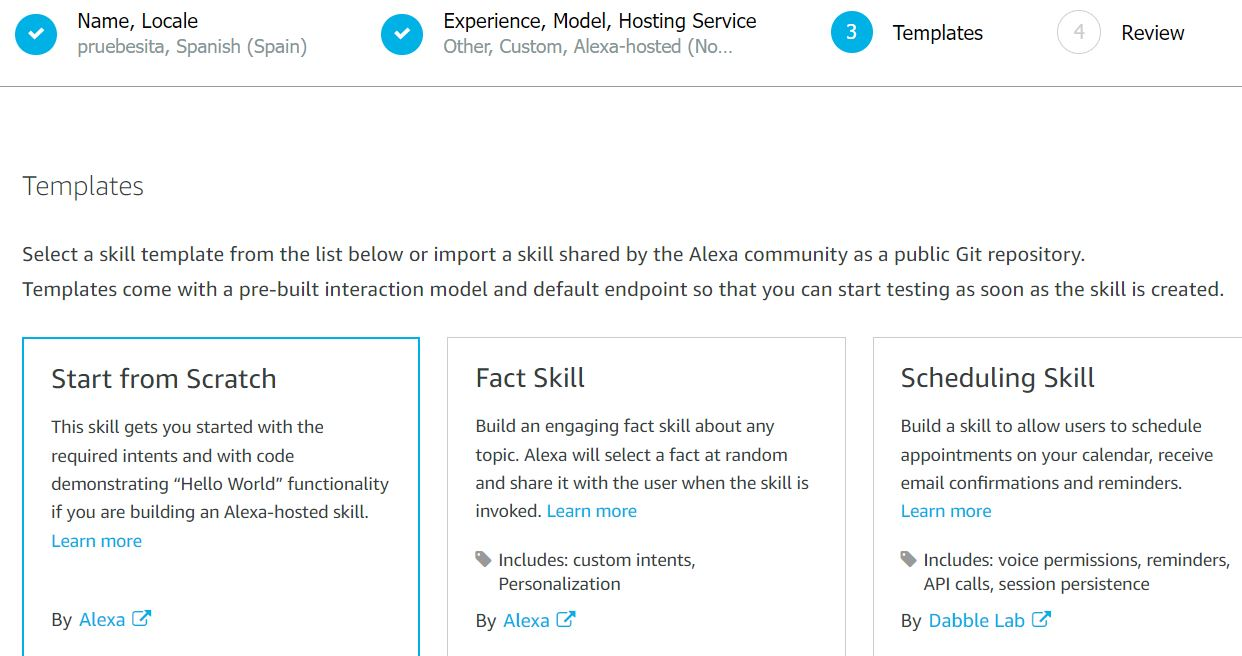
\includegraphics[width=1\textwidth]{imgs/alexa-dev-console-2.jpg}
	\caption{Menú de creación de una skill de Alexa}
	\label{fig:alexa-dev-console-2}
\end{figure}

Una vez creada y finalizada la configuración básica, se abrirá automáticamente el menú de \textit{Build}, desde el que se pueden ajustar varios aspectos de la skill.

Lo primero es declarar el nombre de invocación, que es con el que se llamará a la función de lanzamiento en el momento en el que se abre la skill, y se puede ajustar desde el menú lateral de \textit{Invocations}. Alexa establece una serie de restricciones sobre este parámetro: no puede incluir artículos o preposiciones, debe componerse de mínimo dos palabras, si contiene números estos deben ser escritos de manera completa, no debe incluir mayúsculas ni palabras reservadas como \enquote{Alexa, skill, app,} etc. 

El nombre de invocación elegido es \enquote{probando oca}, por tanto cuando se quiera iniciar la skill, habrá que decir: \enquote{Alexa, abre probando oca}.

Otro elemento desplegable revelante del menú lateral es el modelo de interacción (\textit{Interaction Model}), donde se definen los \textit{intents}. Inicialmente hay cinco predeterminados, de los cuales cuatro son de carácter obligatorio y por tanto no pueden borrarse:

\begin{itemize}
	\item \textbf{AMAZON.CancelIntent}: cancela la acción actual y termina la interacción con la skill.
	\item \textbf{AMAZON.HelpIntent}: proporciona información sobre cómo usar la habilidad.
	\item \textbf{AMAZON.StopIntent}: detiene la acción en curso y finaliza la interacción con la skill.
	\item \textbf{AMAZON.NavigateHomeIntent}: regresa al inicio de o a la pantalla principal.
	\item \textbf{HelloWorldIntent}: ejecuta la acción personalizada predefinida, que consiste en saludar a la persona usuaria. Es la única que puede eliminarse.
\end{itemize}

También se puede acceder y modificar el archivo JSON del modelo de interacción directamente, aunque es aconsejable utilizar en lugar de ello la interfaz de configuración, ya que cada vez que se monta la skill este fichero se actualiza automáticamente.

Otro elemento interesante son los Assets, que permiten la creación de tipos personalizados de slots, la consulta del historial de compilación de la skill y la configuración del \textit{endpoint}. 

Al tratarse de una skill alojada por Alexa, el endpoint se trata de la función Lambda de AWS encargada de la ejecución del código de la skill. Además, por defecto se dispone de tres de ellos, localizados en distintas regiones del mundo: Virginia del Norte, Irlanda y Oregon.

\begin{figure}[H]
	\centering
	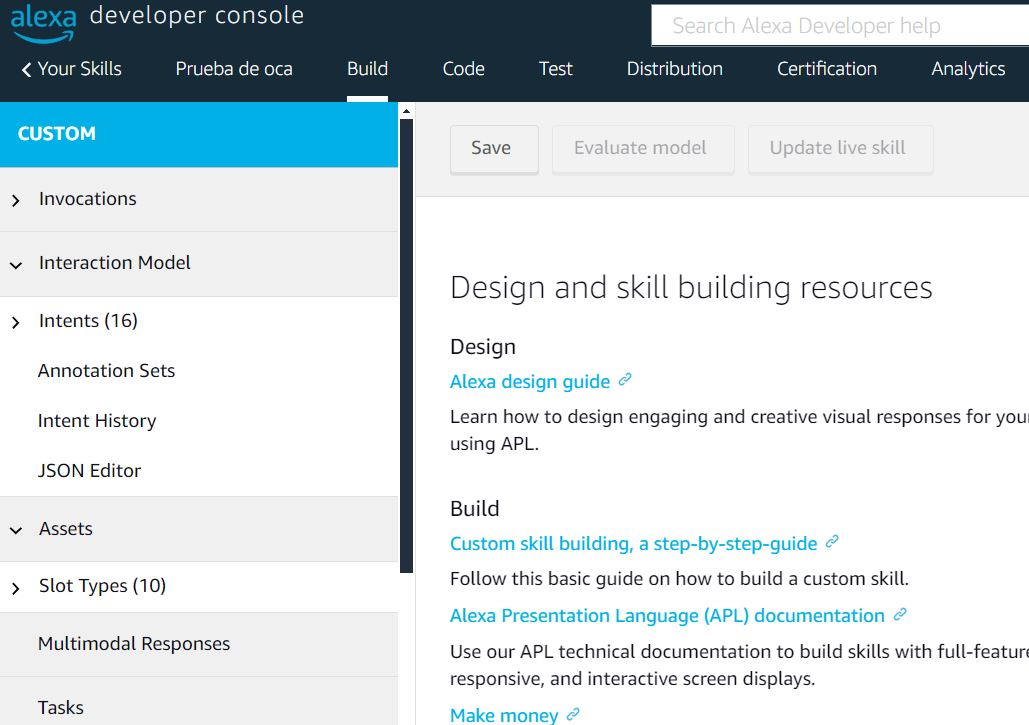
\includegraphics[width=1\textwidth]{imgs/alexa-dev-console-1.jpg}
	\caption{Menú principal de montaje de la skill de Alexa}
	\label{fig:alexa-dev-console-1}
\end{figure}

Si se navega al menú de código desde la barra de herramientas, se puede encontrar la siguiente estructura de archivos:

\begin{figure}[H]
	\centering
	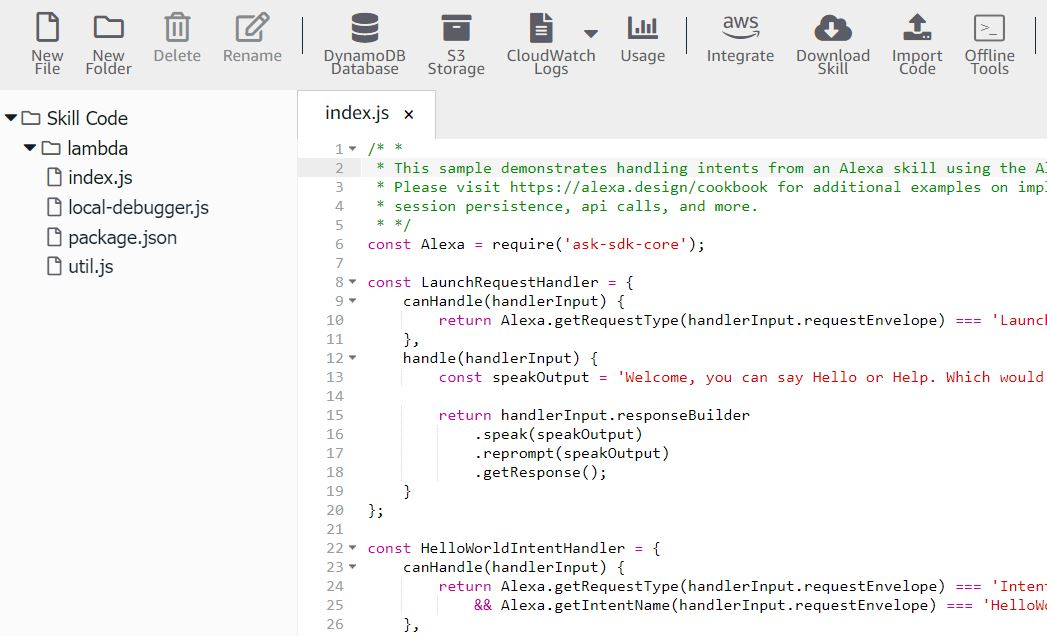
\includegraphics[width=1\textwidth]{imgs/alexa-dev-console-3.jpg}
	\caption{Menú del código de la skill de Alexa}
	\label{fig:alexa-dev-console-3}
\end{figure}

El fichero \textit{index.js} es el más importante, ya que actúa como entrypoint o punto de entrada de la skill, donde se exporta la función de Lambda. Es el que gestiona todos los handlers (manejadores de solicitudes), que determinan el flujo de conversación de Alexa gracias a la capacidad de establecer respuestas concretas a cada intent. Los handlers predefinidos son:
\begin{itemize}
	\item \textbf{LaunchRequestHandler}:  se activa cuando se abre la skill sin especificar un comando, respondiendo con un mensaje de bienvenida.
	\item \textbf{HelloWorldIntentHandler}: responde cuando el usuario invoca a \textit{HelloWorldIntent}, que se limita a saludar.
	\item \textbf{HelpIntentHandler}: maneja el \textit{AMAZON.HelpIntent}, puede invocarse cuando se necesita ayuda.
	\item \textbf{CancelAndStopIntentHandler}: gestiona \textit{AMAZON.CancelIntent} y \textit{AMAZON.StopIntent}, que sirve para detener la skill.
	\item \textbf{FallbackIntentHandler}: se activa se dice algo que no coincide con ninguno de los intents definidos.
	\item \textbf{SessionEndedRequestHandler}: se invoca cuando una sesión termina, ya sea por un comando de usuario o error.
	\item \textbf{IntentReflectorHandler}: útil para la depuración de la skill, ya que responde con el nombre del intent con el que fue llamado. 
	\item \textbf{ErrorHandler}: sirve para la captura de errores de cualquier tipo.
\end{itemize}

Otro archivo esencial en cualquier proyecto realizado con Node.js es \textit{package.json}, donde se definen las dependencias y bibliotecas requeridas, además de permitir la configuración de scripts, pruebas e información acerca de la versión, nombre del proyecto, etc.

Por otro lado, los dos ficheros restantes (\textit{local-debugger.js} y \textit{util.js}) no han sido necesarios para el desarrollo del proyecto, pero pueden servir como base para facilitar la depuración local de la skill y definir funciones de utilidad generales.

\subsection{Configuración de servicios de AWS}

\begin{figure}[H]
	\centering
	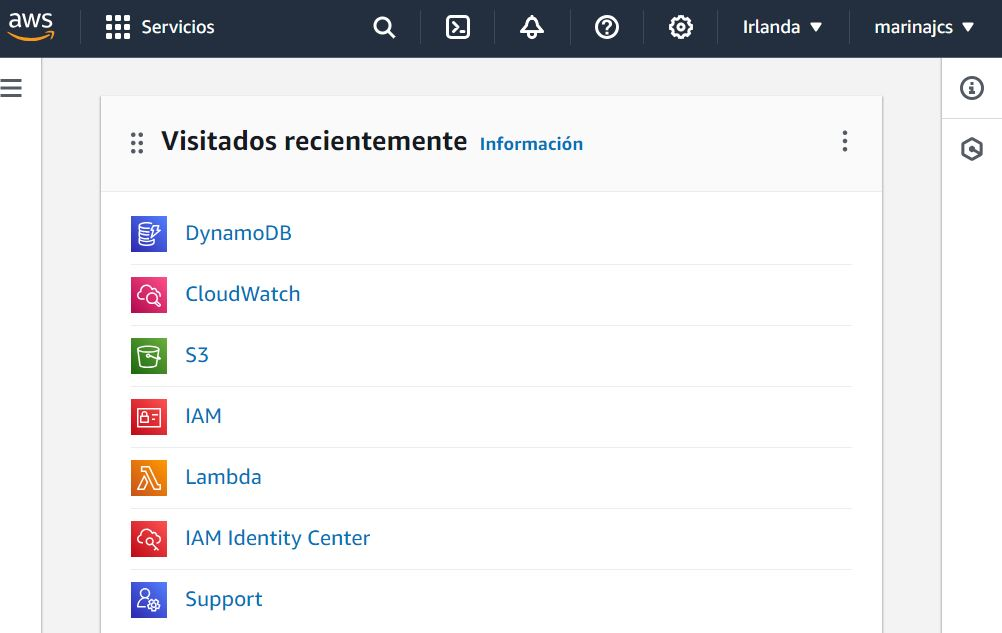
\includegraphics[width=1\textwidth]{imgs/aws-console-1.jpg}
	\caption{Menú de la consola de desarrolladores de AWS}
	\label{fig:aws-console-1}
\end{figure}


\subsubsection{Identity and Access Management (IAM)}

\begin{figure}[H]
	\centering
	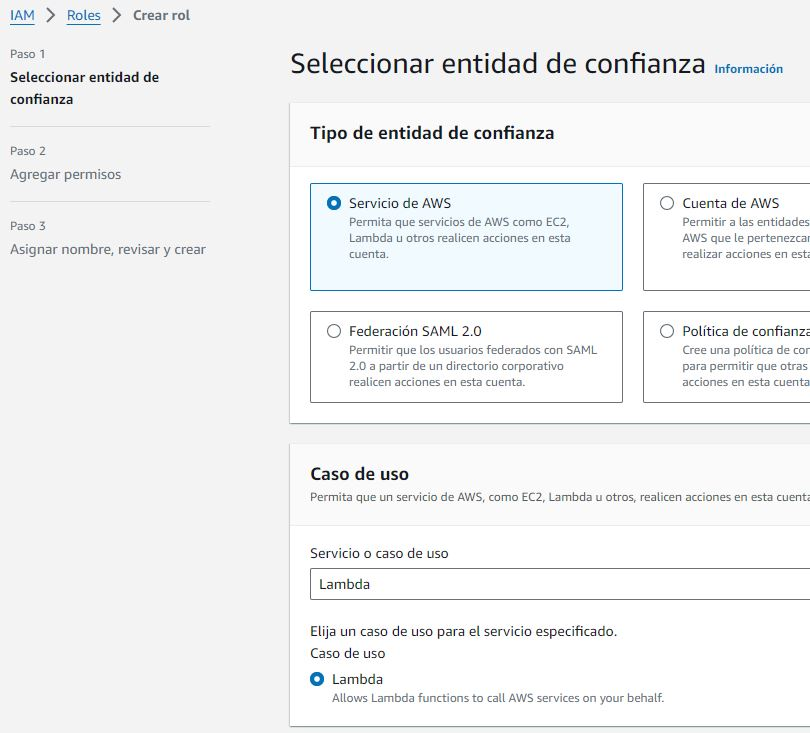
\includegraphics[width=1\textwidth]{imgs/aws-iam-2.jpg}
	\caption{Menú de creación de un rol IAM}
	\label{fig:aws-iam-2}
\end{figure}

Se ha creado un rol de IAM con la finalidad de otorgar permisos temporales de operaciones de DynamoDB a la skill que se está desarrollando.

\begin{figure}[H]
	\centering
	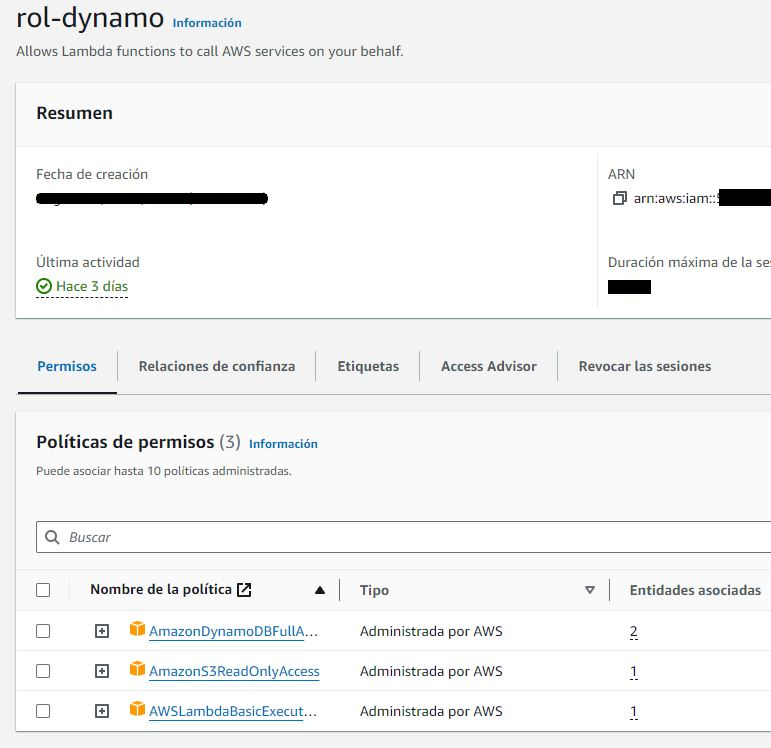
\includegraphics[width=1\textwidth]{imgs/aws-iam-1.png}
	\caption{Rol creado para la skill y sus permisos en AWS}
	\label{fig:aws-iam-1}
\end{figure}

Para que la skill pueda usar los recursos de AWS que será definidos en las secciones siguientes, se necesita modificar el fichero JSON que especifica las relaciones de confianza del rol. Para ello, se añade la siguiente entrada:

\begin{figure}[H]
	\centering
	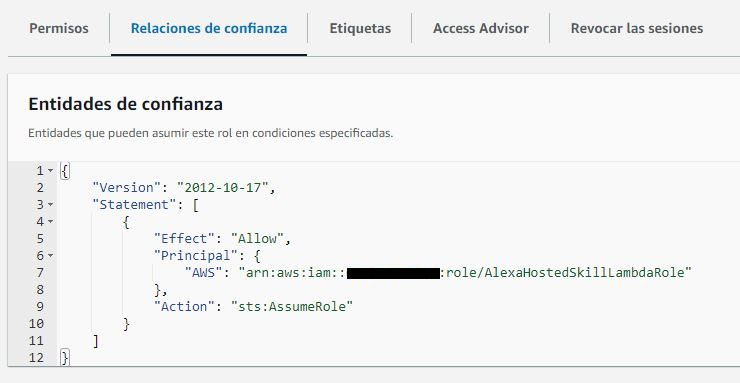
\includegraphics[width=1\textwidth]{imgs/aws-iam-3.png}
	\caption{Configuración de las relaciones de confianza del rol}
	\label{fig:aws-iam-3}
\end{figure}

El texto censurado es el ARN (Amazon Resource Name) o identificador del rol de ejecución IAM que la función Lambda asume al ejecutarse la skill de Alexa. Este se puede obtener desde la consola de desarrolladores de Alexa, en el menú del código, con la opción \textit{Integrate}, especialmente diseñada para poder vincular la skill a servicios personales de AWS.

\begin{figure}[H]
	\centering
	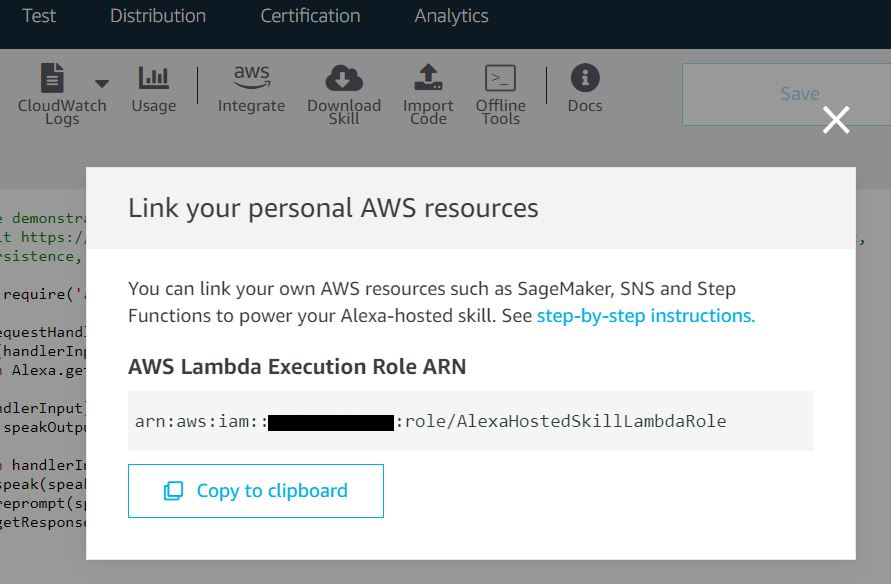
\includegraphics[width=1\textwidth]{imgs/aws-iam-4.png}
	\caption{El AWS Lambda Execution Role ARN de la skill}
	\label{fig:aws-iam-4}
\end{figure}

\subsubsection{Amazon Simple Storage Service (S3)}

Como su nombre indica, es un servicio ofrecido en AWS que permite almacenar objetos de diversos tipos (textos, binarios, documentos, audios, comprimidos, etc). Sin embargo, dados los requisitos de este juego, solo será necesario guardar lo siguiente: las imágenes asociadas a cada casilla, la de la pantalla de bienvenida y los vídeos con las animaciones de los lanzamientos de dado.

En Amazon S3, se ha adoptado el término de \textit{bucket} como un contenedor para almacenar objetos. Cada bucket tiene un nombre único y puede simular una estructura de directorios, además pueden ser de acceso público o privado, al igual que sus elementos, que pueden configurarse a través de políticas de acceso.

Para este proyecto, se ha creado un bucket de nombre \textit{bucket-oca} para guardar todos los archivos multimedia que necesita la skill.

\begin{figure}[H]
	\centering
	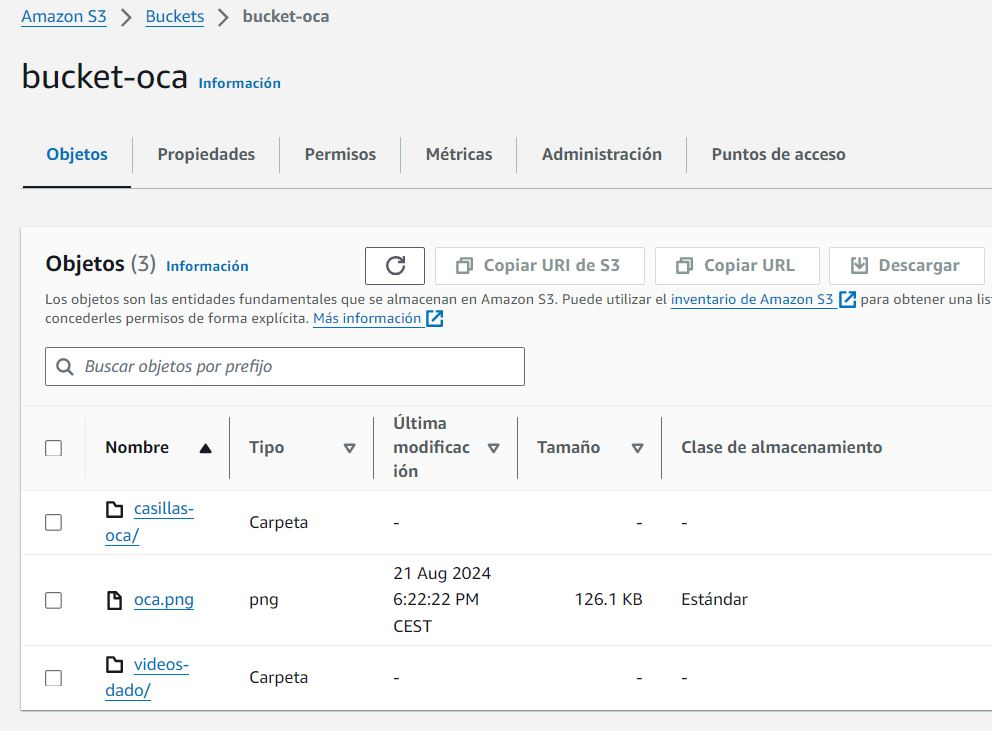
\includegraphics[width=1\textwidth]{imgs/aws-s3-1.jpg}
	\caption{Bucket de Amazon S3 para la skill de la oca}
	\label{fig:aws-s3-1}
\end{figure}

\subsubsection{DynamoDB}

Como se ha mencionado en la sección 6.X, los datos de una skill no persisten de una sesión a otra, por lo que es necesario un mecanismo para guardarlos. Aquí entra el papel de las bases de datos, en particular DynamoDB, también intergado en AWS.

Esta base de datos es de tipo NoSQL y es una alternativa interesante no solo por su total compatibilidad con las herramientas actuales del proyecto debido a que es otro servicio Amazon, sino también por su alta capacidad de adaptación a cualquier volumen de datos. 

Es conocido por optimizar sus tiempos de respuesta y llevar a cabo un escalado automático en función del tráfico, gracias a su esquema NoSQL, cuyos elementos de las tablas se identifican mediante claves primarias únicas. Estas últimas pueden ser de partición o compuestas (unión de una clave de partición con una de ordenamiento).



\subsection{Implementación y estructura del código}



- Alexa Developer Console
+ Config. skill
+ Simulador Alexa

- APL
+ docs
+ envío datasources

- Estructura del código (carpetas, ficheros, funciones, etc)

\subsection{Pruebas}
- hacer tablas
+ nombre prueba
+ descripción
+ respuesta esperada
+ validación
+ correspondencia CU

\subsection{Seguridad}

La seguridad es uno de los requisitos no funcionales más importantes, junto con la usabilidad. Si bien es cierto que en un juego de la oca no se tratan datos de alta importancia que haya que cifrar, es una skill que hace uso de servicios de \textit{Amazon Web Services} (AWS). Estos últimos están vinculados a una cuenta administradora que gestiona los métodos de pago de los servicios cuando estos superan una determinada cuota de uso. Por tanto, para proteger estos servicios y limitar su uso a skills personalizadas concretas, es necesario controlar quién tiene acceso, siguiendo el principio de mínimo privilegio. Esto puede lograrse de forma eficiente mediante los roles de \textit{Identity and Access Management} (IAM).

Estos roles son similares a los usuarios IAM, en el sentido de que permite gestionar el acceso a determinados servicios de AWS de forma centralizada; sin embargo, es más conveniente ya que en lugar de estar asociada a una única entidad, proporciona credenciales a cualquier persona usuaria con duración de una sesión. Además, facilitan el seguimiento de registros (o \textit{logs}) de acciones entre usuarios y servicios.

%https://docs.aws.amazon.com/IAM/latest/UserGuide/id_roles.html
importancia de los roles para la administración de acceso y la seguridad en AWS.

Aunque Amazon ofrece los servicios de DynamoDB y Amazon S3 de manera gratuita para las Alexa-hosted skills, no es sin limitaciones: solo puede crearse una tabla en Dynamo y hay un límite de almacenamiento y operaciones para el bucket de S3. Es por este motivo que se ha optado expandir los recursos de la skill con dichos servicios alojados en una cuenta personal de AWS. 

Para ello, se han seguido los pasos detallados en la doucmentación oficial de Alexa Developer:

https://developer.amazon.com/en-US/docs/alexa/hosted-skills/alexa-hosted-skills-personal-aws.html
